For our results, we executed a backtest over the test set, without transaction costs included. The weigthing of any investment was done proportional to the predicted return, if a return was predicted to be 1.5, there would be a greter proportional investment than in assets where the return was predicted to be 0.5. If the predicted return was negative, no investment was made. At any given timestep, the entir eportfolio was allocated. 

\begin{center}
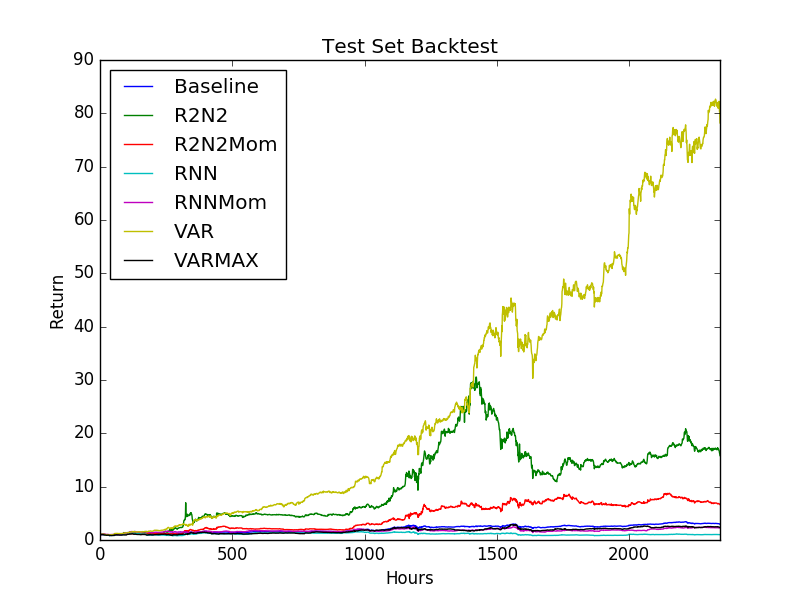
\includegraphics[scale = 0.6]{Results/backtest_all.png}
\end{center}

The visual of the backtest is seen in the figure above, and the results can be found in the table below.

\begin{tabular}{lrrrrr}
\toprule
{} &       auc &     return &    sharpe &       mse &  max\_drawdown \\
\midrule
Baseline &  0.500000 &   1.939799 &  2.886800 &  0.999415 &      0.292192 \\
R2N2     &  0.506587 &  14.827861 &  2.064562 &  0.000478 &      0.643012 \\
R2N2Mom  &  0.501317 &   5.641210 &  2.216578 &  0.000470 &      0.283592 \\
RNN      &  0.498271 &  -0.012393 & -0.067288 &  0.002232 &      0.490028 \\
RNNMom   &  0.501635 &   1.235352 &  4.249862 &  0.000472 &      0.437239 \\
VAR      &  0.542329 &  77.204319 &  3.145382 &  0.000472 &      0.332267 \\
VARMAX   &  0.498495 &   1.359462 &  2.640301 &  0.000478 &      0.442717 \\
\bottomrule
\end{tabular}


